\documentclass[10pt,twocolumn,letterpaper]{article}

\usepackage{cvpr}
\usepackage{times}
\usepackage{epsfig}
\usepackage{graphicx}
\usepackage{amsmath}
\usepackage{amssymb}
\usepackage[pagebackref=true,breaklinks=true,letterpaper=true,colorlinks,bookmarks=true,bookmarksnumbered=true,hypertexnames=false,linkbordercolor={0 0 1}]{hyperref}

\cvprfinalcopy

\def\httilde{\mbox{\tt\raisebox{-.5ex}{\symbol{126}}}}

\ifcvprfinal\pagestyle{empty}\fi
\begin{document}

%%%%%%%%% TITLE
\title{Deep Neural Nets for Handwritten Digit Classification}

\author{Anusha Dasarakothapalli\\
University of Wisconsin - Madison\\
{\tt\small anusha@cs.wisc.edu}
\and
Gautam Umesh Sargur\\
University of Wisconsin - Madison\\
{\tt\small gautam@cs.wisc.edu}
}

\maketitle
\thispagestyle{empty}
%%%%%%%%% ABSTRACT
\begin{abstract}
   For a few years now, the problem of identifying digits from handwritten documents has become an important one especially when it comes to digitization of old records. We have implemented a digit recognition engine using a multi-layered perceptron (MLP) and a support vector machine to classify handwritten images. We have evaluated the performance of the deep network in different settings changing the number of hidden layers and compared it to a single layer neural network. We have also presented the results of using an SVM for the same classification problem using both linear and RBF kernels. The Deep neural networks are evaluated by cross-validation and a paired t-test.
\end{abstract}

%%%%%%%%% BODY TEXT
\section{Introduction}

It is well known that training multi-layered neural networks is very difficult. The standard approach is to assign arbitrary weights to the network and applying gradient descent using backpropagation. But, this could lead to very poor solutions for networks with more than 3 hidden layers. For this reason, the most widely used deep networks have a maximum of two hidden layers. Deep networks have been used for a number of image classification applications like \cite{Schmidhuber:2012:MDN:2354409.2354694}.\\

Researchers worldwide have been endeavouring to integrate the gathered terabytes of handwritten images into a digital library. Our database consists of 10 classes (digits from 0 to 9). Typically, there are two main approaches to solve multi class problems in machine learning: generative model-based and SVM-based. We take advantage of both these approaches and pick the deep neural net from the former and use the Support Vector Machine from the latter.\\

In this paper, we describe two approaches to classify hand written images. We have implemented variants of the deep network with 2, 3 and 4 hidden layers and have compared the results to a traditional single layer neural net and the state-of-the-art digit recognition classifier.  In addition to this, we have used LIBLINEAR\cite{REF08a} and LIBSVM \cite{CC01a} SVM for the same classification and presented the results. We have finally evaluated the neural network approach using 10-fold cross validation and a paired t-test.\\

The structure of this paper is organized as: Section 2 reviews the work done in the field of image recognition using a variety of classification models. Section 3 describes our proposed approaches for digit recognition. Section 4 discusses the analysis of our approach, Section 5 presents our findings, lists the advantages and disadvantages of each approach and describes the future work and section 6 concludes the paper.
\begin{figure*}
\label{fig:structure}
\begin{center}
	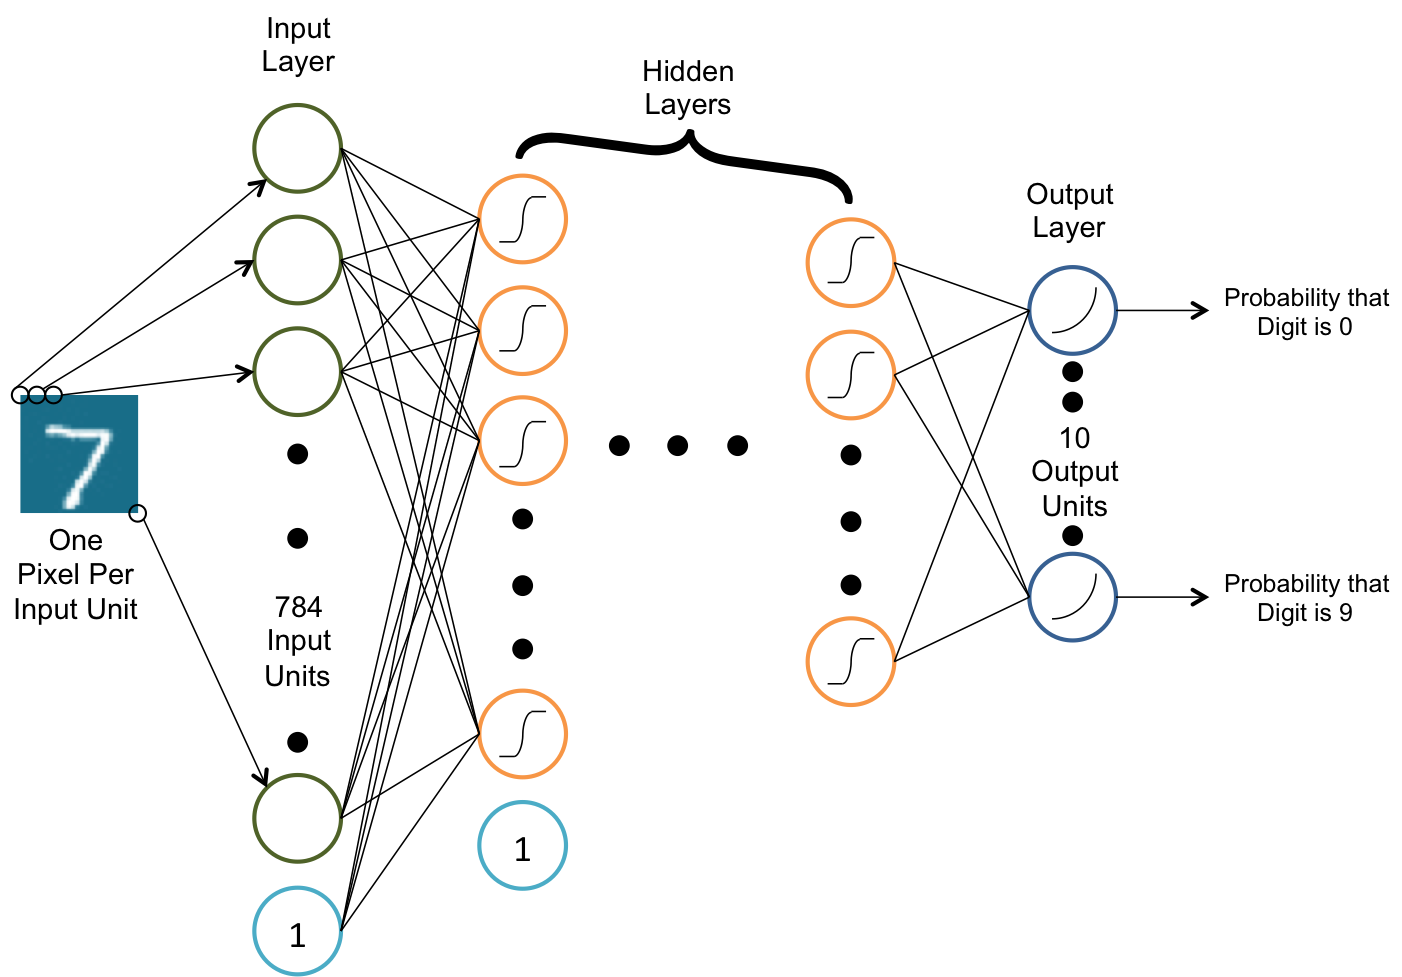
\includegraphics[scale=0.7]{../images/Network.png}
\end{center}
   \caption{The basic structure of all networks used in this project}
\end{figure*}

\section{Related Work}
A lot of research has been done in the field of hand-written digit recognition. Using deep neural networks for this purpose has both advantages and disadvantages. Because of many levels of non-linearities, they can compactly represent highly non-linear and highly varying functions \cite{Larochelle:2009:EST:1577069.1577070}. Hinton et al \cite{Hinton:2006:FLA:1161603.1161605} proposed a greedy, layer-wise learning procedure relying on the training algorithm of restricted Boltzmann machines (RBM) to initialize the parameters of a deep belief network, a generative model of many layers of hidden causal variables. Deep architectures can be much more efficient (sometimes exponentially) than shallow architectures, in terms of computational elements and parameters required to represent some functions. An approach that was considered was to constructively add layers, where each layer can be seen as a representation of the input obtained through a learned transformation.\\

The authors of \cite{Fahlman:1990:CLA:109230.107380} used a supervised criterion at each stage. However, this may be too greedy and might not yield as good generalization as an unsupervised criterion. One more issue that was observed with using deep neural networks for image classification was that training them requires a long time on CPU. Hence, to train huge deep networks, \cite{Schmidhuber:2012:MDN:2354409.2354694} implemented them on GPUs building upon the work of \cite{Ciresan:2010:DBS:1943016.1943024} and \cite{Ciresan:2011:FHP:2283516.2283603}. They also show that properly trained wide and deep neural networks can outperform all previous methods and they demonstrate that unsupervised initialization or pre-training is not necessary. Other research \cite{Lee:2009:CDB:1553374.1553453} done in this field presented a convolutional deep belief network which scales to realistic image sizes. They also observed that using deep neural networks to classify images can be challenging because of two important reasons: images are high-dimensional so the algorithms must scale gracefully and be computationally tractable even when applied to large images, objects can appear at arbitrary locations in images. A three-layer network is used where the layers each learn edge detectors, object parts and objects respectively. They achieved a 0.8\% test error. Another approach \cite{NIPS2012_4824} trained one of the largest convolutional neural networks till date, on the subsets of ImageNet. A highly optimized GPU implementation of 2D convolution and all other operations inherent in convolutional deep nets.

\section{Our Approach}
\subsection{The Dataset}
The MNIST database of handwritten digits has a training set of 60,000 examples, and a test set of 10,000 examples. It is a subset of a larger set available from NIST. The digits have been size-normalized and centred in a fixed-size image. Each of the images in the training and test set are gray scale images with dimensions of 28 pixels wide by 28 pixels high.\\

The MNIST database was constructed from NIST's Special Database 3 (SD-3) and Special Database 1 (SD-1) which contain binary images of handwritten digits from about 500 authors. The MNIST training set is composed of 30,000 patterns from SD-3 and 30,000 patterns from SD-1. The test set is composed of 5,000 patterns from SD-3 and 5,000 patterns from SD-1. The 60,000 pattern training set contain examples from approximately 250 writers. Care has been taken to ensure that the set of writers of the training set and test set are disjoint.

\subsection{Deep Neural Network Approach}
Deep Neural Networks are basically like any other Artificial Neural Network but more than one hidden layer. The conventional methods of training an ANN will not work well with deeper architectures for two main reasons. (1) The objective function in case of deep networks is not smooth and the algorithm has a tendency to get stuck in a local minima. (2) The gradient calculated becomes very small in deeper layers of the network. Therefore, our approach involves the training the Neural Network in a layer-wise fashion followed by one round of back-propagation on the entire network. This sequential training process turns out to be better because it is believed that the layer-wise training gives a good starting point for the back-propagation algorithm to converge to a global optima though there is no theoretical proof to substantiate this claim.

\subsubsection{The Structure of the Network}
All networks used in our project have certain common aspects that they share. The inputs layer of the network consists of 784 units. Each of these units correspond to a pixel in an image. All values are normalized to be within the range [0,1] to alleviate the effects that large values in the original range of [0,255] will have on the computation.\\

The input layer is followed by two or more hidden layers. All units in the hidden layers compute their output values using the \textit{sigmoid} activation function. $$f(x) = \frac{1}{1+e^{w^Tx}}$$ where, $w$ is the vector of weights from the previous layer to the current one and $x$ is the output of the previous layer.\\

The hidden layers are followed by an output layer with ten units one each for the ten classes that we want to classify the input data into. All units in the output layer compute their output values using the \textit{softmax} activation function. $$f_i(x) = \frac{e^{w_i^Tx}}{\displaystyle\sum\limits_{j=1}^{10} e^{w_j^Tx}}$$ where, i $\in$ [1,10] and each $f_i$ represents the output of unit $i$ in the output layer, $w_i$ represents the vector of weights from the previous layer to unit $i$ and $x$ is the output of the previous layer. The value at each output unit represents the probability that the given input image belongs to that particular class. The unit with the highest probability is considered to best represent the class to which the image belongs. This structure is clearly shown in Figure (\ref{fig:structure}).

\subsubsection{Autoencoders and Unsupervised Features}
An autoencoder neural network is an unsupervised learning algorithm that applies back-propagation, setting the target values to be equal to the inputs. I.e., it uses $y^{(i)} = x^{(i)}$. At this phase, all labels are ignored. Since, we are not using any labels, out expectation at this stage is that the hidden layer will be able to learn some features from the input data that is a somewhat more abstract representation of the input and therefore helps in better predictions that if just the raw input values were to be used. This, in fact, turns out to be true and we can visualize the weights learned at this stage to see that the network has learned features akin to strokes that represent curvatures in the digit. This result is shown in the Figure (\ref{fig:weights}).
\begin{figure}[t]
\begin{center}
   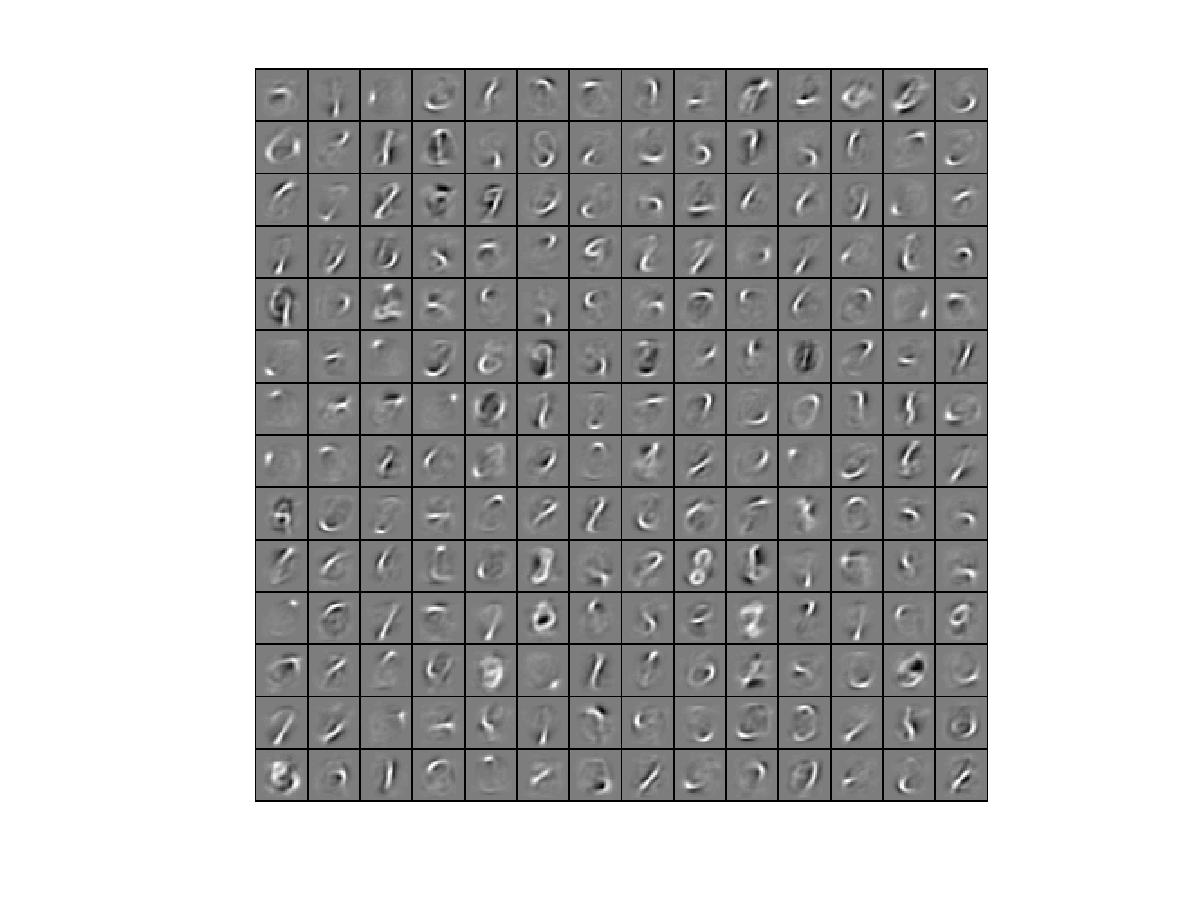
\includegraphics[width=1\linewidth]{../images/weights.jpg}
\end{center}
   \caption{Visualization showing values of weights grouped into 196 images each of height 28 pixels and width 28 pixels. As it can be seen, one layer of autoencoder training has learned pen-stroke like features from the input images.}
   \label{fig:weights}
\end{figure}

In autoencoder training, we follow the batch learning approach over on-line learning as it is easier to implement in matlab and boils to a few matrix multiplication operations. The cost function $C$ for this step looks like this.
\begin{multline*}
C(W,b) = \left[\frac{1}{m}\displaystyle\sum\limits_{i=1}^m \left(\frac{1}{2}\|h_{W,b}(x^{(i)})-y^{(i)}\|^2_2\right)\right]\\
+\frac{\lambda}{2}\sum\limits_{l=1}^{n_l-1}\sum\limits_{i=1}^{s_l} \sum\limits_{j=1}^{s_{l+1}} (W_{ji}^{(l)})^2
\end{multline*}
where, $m$ is the number of training examples, $h_{W,b}$ are the activations of the output layer, $\lambda$ is the weight decay coefficient, $n_l$ id the number of layers, $s_k$ the number od units in layer $k$ and $W_{ji}^{(l)}$ is the weight from unit $j$ in layer $l$ to unit $i$ in $l+1$. The first term calculates the sum of squared error and the second term, called the \textit{weight decay} term, is used to decrease the values of the weights and hence prevent over-fitting. The goal is to minimise this cost function and we use the \textbf{L-BGFS} algorithm for this instead of conventional gradient descent as it is faster and more accurate.\\

The above cost function works well for small number of hidden units and tends to produce bad results as the number of hidden units increase in number. Therefore, in addition to the above cost function, we would also like to enforce a sparsity constraint. This means that we want the average activation at each unit to be nearly zero. This is enforced by selecting a value $\rho$ which specifies the desired average activation in each hidden unit. The improved cost function now looks like this. $$C_{sparse}(W,b) = C(W,b) + \beta\displaystyle\sum\limits_{j=1}^{s_l} KL(\rho\|\hat{\rho}_j)$$ where, $s_l$ id the number of units in layer $l$, $\beta$ is used to control the weight of the sparsity term and $\hat{\rho}_j$ is the activation at unit $j$. The KL term represents the Kullback-Leibler divergence between Bernoulli distributions with mean $\rho$ and $\hat{\rho}_j$ and looks like this.
$$KL(\rho\|\hat{\rho}_j) = \rho\log\frac{\rho}{\hat{\rho}_j} + (1-\rho)\log\frac{1-\rho}{1-\hat{\rho}_j}$$
Therefore, this new sparse cont function is minimized using \textbf{L-BGFS}. It is necessary to compute gradients for these functions but this is a simple enough task and we do not present the derivation here in the interest of conserving space.

\subsubsection{Stacked Autoencoders}
As mentioned at the beginiing of this section, each layer is trained as an sparse autoencoder and the output layer is discarded. The output of the trained hidden layer is used as the input (and by extension as the output as we are training autoencoders) for the next layer to be trained. This process is repeated for the number of specified hidden layers and a softmax regression layer is added to the last hidden layer to classify the input images using supervised learning.

\subsubsection{Softmax Regression in Output Layer}
The output layer in out implementation consists of ten softmax units. We use this approach for this multi-class problem instead of a one-vs-rest approach which involves training ten classifiers and is hence time consuming. The softmax function gives a natural and intuitive way to represent the output as a probability of input belonging to a particular class. As with the autoencoders, we use batch learning instead of on-line learning to train theis layer as well. The cost function $C$ for this layer looks as follows.
\begin{multline*}
C(W) = \left[-\frac{1}{m}\sum\limits_{i=1}^m \sum\limits_{j=1}^k 1\{y^{(i)} = j\} \log \frac{e^{w_i^Tx^{(i)}}}{\sum_{l=1}^{k} e^{w_l^Tx^{(i)}}}\right]\\
+ \frac{\lambda}{2}\sum\limits_{i=1}^k \sum\limits_{j=0}^{s_l} (W_{ij})^2
\end{multline*}
where, $m$ is the number of input images, $k$ is the number of classes (10 in our case), $w_i$ are weight coming in from the last hidden layer to output unit $i$, the function $1\{statement\}$ evaluates to 1 if the $statement$ in it is true and 0 otherwise, $s_l$ is the number of units in the last hidden layer and $x^{(i)}$ is the vector that represents input image $i$. This cost function is similar to the one used in autoencoders in that it has one term to take care of the error in prediction and another for the \textit{weight decay} in order to avoid over-fitting.\\

The cost function is again minimized using \textbf{L-BGFS}. It is necessary to compute the derivative of the cost function and as mentioned before, we do not show the derivation here in the interest of conserving space.

\subsection{The SVM approach}
The state of the art before deep learning came along was the SVM algorithm. In order to compare the results of our Deep learning implementation to the state of the art, we evaluated the dataset using a multiclass implementation of SVM using both the \textit{Radial Bias Function} and the linear kernel. The \textit{Radial Bias Function} looks as follows. $$e^{-\gamma\|x^{(i)}-x^{(j)}\|^2_2}$$ where, $\gamma$ is a parameter and $x^{(i)}$ and $x^{(j)}$ are two input feature vectors. The RBF is especially useful because it maps the input into an infinite dimensional vector. Since the SVM algorithm finds a hyperplane  that separates the positive from the negative examples, a higher dimensional space always tends to yield better results.\\

We used LIBLINEAR to get the SVM model for a linear kernel as it is much faster and is optimized to handle linear SVMs better and faster than LIBSVM. But, as the former does not have any support for non-linear kernels, we use the latter to present results with the RBF. In LIBLINEAR, we used the L2-regularized L2-loss support vector classification as it solves the primal problem which has 784 parameters as opposed to the dual which would have about 60000 parameters to learn. In LIBSVM, we used C-SVC algorithm with the RBF kernel for classification. All input values were normalized to the [0,1] range before being used.
\begin{figure*}
\begin{center}
	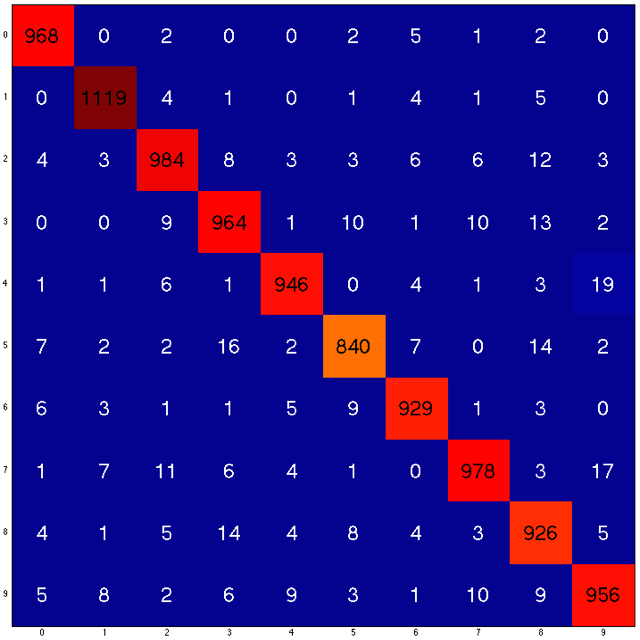
\includegraphics[scale=0.25]{../images/confusion_1.png}
	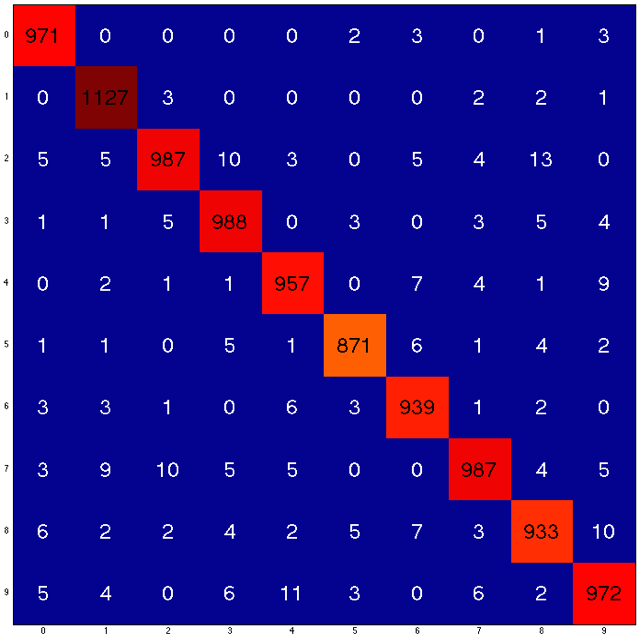
\includegraphics[scale=0.25]{../images/confusion_2_2.png}
	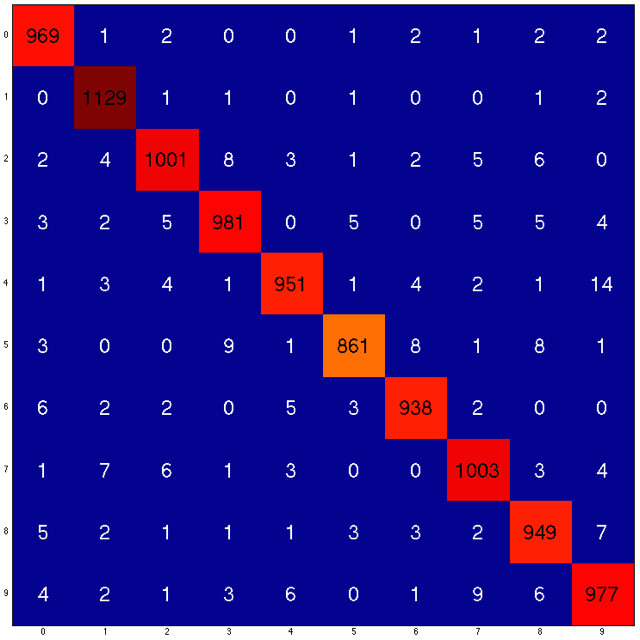
\includegraphics[scale=0.25]{../images/confusion_2_1.png}
	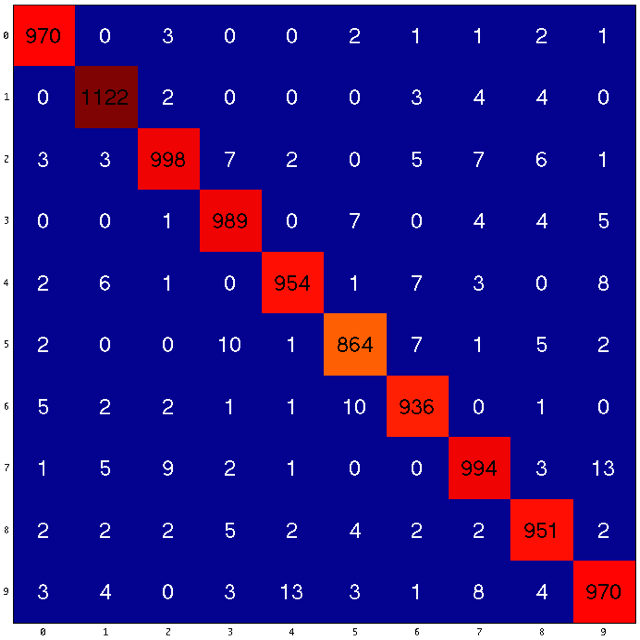
\includegraphics[scale=0.25]{../images/confusion_3.png}
	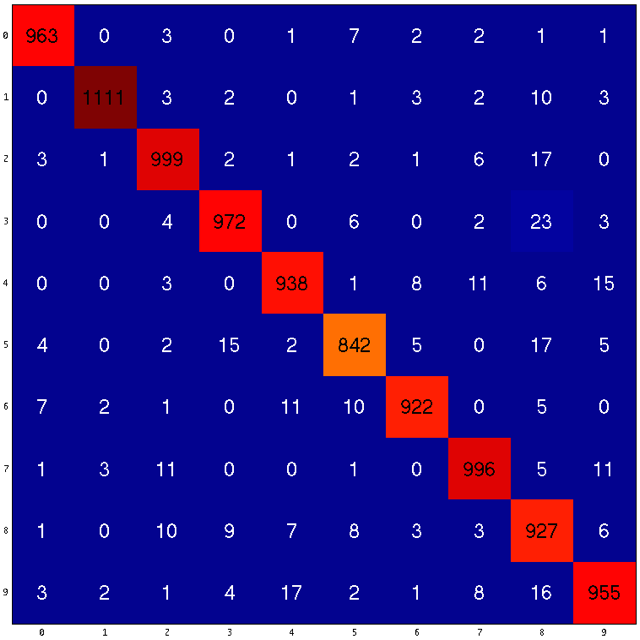
\includegraphics[scale=0.25]{../images/confusion_4.png}
\end{center}
	\caption{Confusion matrices of Network 1(top left), 2(top center), 3(top right), 4(bottom left) and 5(bottom right)}
	\label{fig:confusion}
\end{figure*}
\section{Experiments and Evaluation}
\subsection{Deep Neural Network}
The network topology can be varied greatly and the number of possible combinations of number of number of hidden layers and the number of units in each hidden layer is virtually infinite. We selected four different network topologies with more than one hidden layer to evaluate the performance of the algorithm. In addistion to this, we also ran our algorithm for one hidden layer and we present the results we thus obtained here.
\begin{center}
\begin{tabular}{|c|c|c|}
	\hline
	\textbf{Network \#} & \textbf{\# Hidden Layers} & \textbf{Configuration}\\ \hline \hline
	1 & 1 & 392\\ \hline
	2 & 2 & 500$\rightarrow$200\\ \hline
	3 & 2 & 392$\rightarrow$196\\ \hline
	4 & 3 & 392$\rightarrow$196$\rightarrow$98\\ \hline
	5 & 4 & 392$\rightarrow$196$\rightarrow$98$\rightarrow$49\\ \hline
\end{tabular}
\end{center}
\begin{center}
	Table 1: Network topology for all networks we tested
\end{center}

Table (1) gives details of all networks. We performed a 10-fold cross-validation on each one of these networks followed by significance testing by use of the students t-test on each pair of hypotheses. We will refer to each hypothesis by its number in the above table to avoid repetition.

\subsubsection{Test Set Accuracy and Confusion Matrices}
The performance of each network on the test set is summarised in Table (2). Figure (\ref{fig:confusion}) shows the confusion matrices for all 5 networks. As observed in almost all matrices, the networks tend to get confused between digits that look similar. For Example, 4 and 9 appear to be very similar depending on the handwriting of the individual and so do other pairs of numbers such as 3 and 5, 0 and 6, 8 and 5 and so on. Network 4 seems to perform the best with a peak accuracy of 98.48\% among all tests that were conducted.
\begin{center}
\begin{tabular}{|c|c|}
	\hline
	\textbf{Network \#} & \textbf{Peak Accuracy} \\ \hline \hline
	1 & 96.10\\ \hline
	2 & 97.72\\ \hline
	3 & 98.10\\ \hline
	4 & 98.48\\ \hline
	5 & 97.25\\ \hline
\end{tabular}
\end{center}
\begin{center}
	Table 2: Peak accuracy for each network
\end{center}

\begin{figure*}
\begin{center}
\begin{tabular}{|c|c|c|c|c|c|c|c|c|c|c|c|}
	\hline
	\textbf{Network \#} & \textbf{Fold 1} & \textbf{Fold 2} & \textbf{Fold 3} & \textbf{Fold 4} & \textbf{Fold 5} & \textbf{Fold 6} & \textbf{Fold 7} & \textbf{Fold 8} & \textbf{Fold 9} & \textbf{Fold 10} & \textbf{Average}\\ \hline \hline
	1 & 95.75 & 95.70 & 94.77 & 95.45 & 95.45 & 95.32 & 95.07 & 94.65 & 94.68 & 96.25 & 95.31\\ \hline
	2 & 97.30 & 97.43 & 97.30 & 97.53 & 97.47 & 97.07 & 97.42 & 97.05 & 96.75 & 97.83 & 97.27\\ \hline
	3 & 97.33 & 97.35 & 97.17 & 97.57 & 97.25 & 97.08 & 97.18 & 96.93 & 96.77 & 98.07 & 97.31\\ \hline
	4 & 97.33 & 96.93 & 96.83 & 96.90 & 97.50 & 97.33 & 96.83 & 96.53 & 96.33 & 97.73 & 97.03\\ \hline
	5 & 95.93 & 95.80 & 96.68 & 97.08 & 96.58 & 96.83 & 96.22 & 94.03 & 95.28 & 97.02 & 96.15\\ \hline
\end{tabular}
\end{center}
\begin{center}
	Table 3: Cross validation accuracies and average accuracy for all networks that we tested
\end{center}
\end{figure*}

\subsubsection{Cross Validation}
We did a 10-fold cross validation on each of the 5 networks mentioned above. We only used the 60000 training examples without stratified sampling in each fold of cross validation therefore giving a cross validation training set size of 54000 and a test set size of 6000. The results of this are as shown in Table (3). As it is evident from the results, Network 3 seems to perform the best in cross-validation. All networks seem to perform better than the one layer network as well.

\subsubsection{Paired t-test}
We performed a paired t-test between every pair of networks in Table (1) and the p-values are summarized in a matrix in Table (4). 
\begin{center}
\begin{tabular}{|c|c|c|c|c|c|}
	\hline
	\textbf{Network \#} & \textbf{1} & \textbf{2} & \textbf{3} & \textbf{4} & \textbf{5} \\ \hline \hline
	1 & 1.00 & 0.00 & 0.00 & 0.00 & 0.02\\ \hline
	2 & 0.00 & 1.00 & 0.79 & 0.19 & 0.01\\ \hline
	3 & 0.00 & 0.79 & 1.00 & 0.11 & 0.01\\ \hline
	4 & 0.00 & 0.19 & 0.11 & 1.00 & 0.04\\ \hline
	5 & 0.02 & 0.01 & 0.01 & 0.04 & 1.00\\ \hline
\end{tabular}
\end{center}
\begin{center}
	Table 4: p-values for each pair of network topologies
\end{center}
A p-value of less than 0.01 suggests that the difference the ability of the two hypotheses to classify the data is strongly significant, a p-value between 0.01 and 0.05 suggests moderate significance and anything greater than 0.05 suggests that the two hypothesis are almost similar.\\

From Table (4), we can infer that the network with one hidden layer performs significantly worse than all networks with more than one hidden layer. In addition, we also see that the four layer network performs worse than the other deep networks. This could be because we have only 49 units in the last layer and with the sparsity parameter forcing all activations to be close to $\rho$, there might actually be a reduction in expressive power. To get around this anomaly of deeper networks performing worse than shallower ones, we need to add more units to each layer. Unfortunately the memory requirements and time to train such a network are too high and hence this theory could not be tested.

\begin{figure}[t]
\begin{center}
   	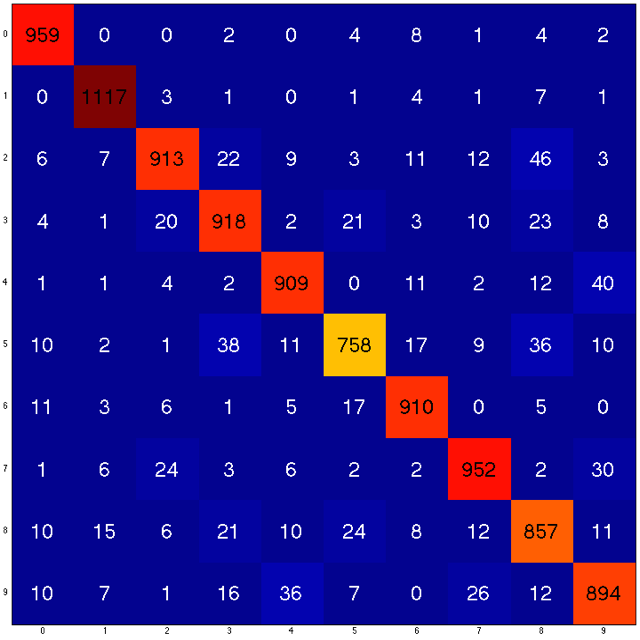
\includegraphics[width=0.65\linewidth]{../images/confusion_svm.png}
	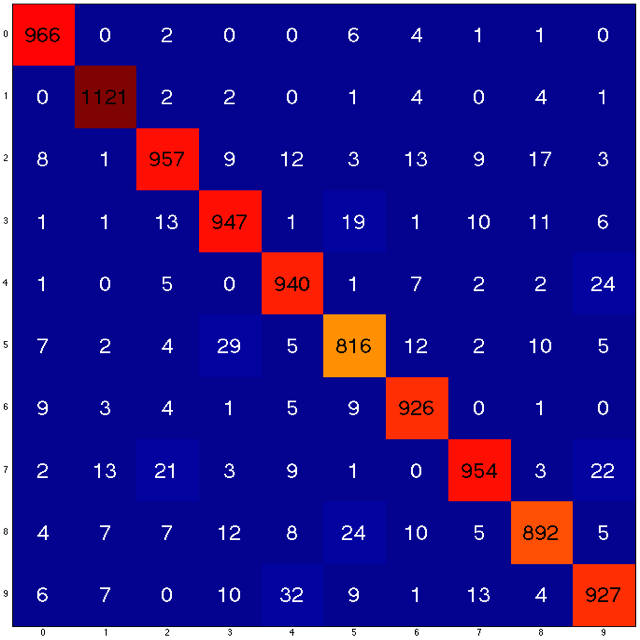
\includegraphics[width=0.65\linewidth]{../images/confusion_svm_rbf.png}
\end{center}
   \caption{Confusion matrices for SVM with linear kernel(top) and RBF kernel(bottom)}
   \label{fig:confusionsvm}
\end{figure}

\subsection{Support Vector Machines}
SVMs were considered to be state of the art before Deep Neural Networks were proposed and hence, we present the results of two runs of the SVM algorithm using a linear and RBF kernel. Figure (\ref{fig:confusionsvm}) shows the confusion matrices for each of these test runs. The linear kernel SVM had a peak test set accuracy of 91.87\%. As mentioned eralier, for the linear kernel we used the primal form of the SVM optimization as it tuns out to be faster. The RBF kernel SVM had a peak test set accuracy of 94.46\%. The value og $\gamma$ used in our experiment was 0.1 and the dual formulation of the SVM optimization was used to solve this problem. We did not perform any cross-validation tests and hence cannot show a significance test for the SVM algorithms and the Deep Networks. But as seen from the confusion matrices and peak accuracy figures, the Deep Networks seem to perform better.\\

As seen in Figure (\ref{fig:confusionsvm}), The SVM algorithms performance is similar to the Deep Network in the sense that both seem to wrongly predict digits that have similar visual appearance. In addition to these understandable mistakes, the SVM also gets confused between digits such as 2 and 8 which are in now way similar in appearance. The RBF kernel somewhat alleviates this problem but is still not accurate enough to compete with Deep Neural Networks.

\section{Future Work}
Although our implementation of the Deep Neural Network show significant improvement in accuracy over single layered neural networks and SVMs, there have been other developments in this area such as Convolutional Neural Nets that provide much better results. The highest accuracy for this dataset is 99.77\% that was obtained using CNNs. Some improvements to this project might involve incorporating some aspects of CNNs to improve the accuracy further. In addition, plain Deep Neural Networks are able to accomplish an accuracy of 99.17\% on this dataset. Another improvement therefore, could be to add more layers and try out bigger networks with hidden layers containing units of the order of 1000s instead of 100s as we have done now.\\

These Algorithms also seem to work better when the training and test images are de-skewed and distorted or rotated. Therefore, applying transforms to input images and increasing the dataset size could also lead to better results.

\section{Conclusion}
The project discusses two approaches to classifying handwritten digits into their respective classes. We have successfully been able to analyze and show how changing either the topology or size of the network have helped in increasing the overall accuracy of the neural network. Our project also involved comparing our implementation of Deep Neural Networks to Support Vector Machines. We also did significance testing across five different network topologies and showed that deeper networks and autoencoder training schemes usually tend to perform better than when  conventional single layer networks and back-propagation are used for classification.
\subsection*{Acknowledgement}
We would like to thank Prof. David Page for providing his valuable input for this project and the tutorial by Andrew Ng \cite{ANg13t} which we used as a reference for implementing our Deep Neural Net.

{\small
\bibliographystyle{ieee}
\bibliography{egbib}
}

\end{document}
